\chapter{Connectors}\label{sec:connector}

The UCANPHY standard defines several connector types optimized for different applications:
from highly compact systems to large deployments, from low-cost to safety-critical applications.
Each connector type specification includes an integrated power supply interface
(section~\ref{sec:power}).

Implementations should provide two identical parallel connectors for each CAN interface per device
instead of relying on T-connectors.
T-connectors should be avoided because typically they increase the stub length, weight, and
complexity of the wiring harnesses.
All signals of the paired connectors, including those that are unused, shall be interconnected one to one.

\begin{UAVCANSimpleTable}[wide]{Standard UAVCAN/CAN connector types}{|l l l X|}\label{table:connector_summary}
    Connector name & Base connector type & Integrated power & Known compatible standards \\
    \textbf{UCANPHY D-Sub} &
    Generic D-Subminiature DE-9 &
    24 V, 3 A &
    De-facto standard connector for CAN, supported by many current specifications. \\

    \textbf{UCANPHY M8} &
    Generic M8 5-circuit B-coded &
    24 V, 3 A &
    CiA 103 (CANopen) \\

    \textbf{UCANPHY Micro} &
    JST GH 4-circuit &
    5 V, 1 A &
    Dronecode Autopilot Connector Standard \\
\end{UAVCANSimpleTable}

\clearpage  % Enforce \clearpage because the text here is very graphics-heavy and may be hard to read otherwise
\section{UCANPHY D-Sub}

The UCANPHY D-Sub connector type is based upon, and compatible with, the D-Subminiature DE-9 CAN connector
(this is the most popular CAN connector type, in effect the de-facto industry standard).
This connector is fully compatible with CANopen and many other current specifications.

{
\NoLeftSkip
\begin{UAVCANCompactTable}{|X[2] X|}
    Advantages & Disadvantages \\
    \begin{itemize}
        \item Highest level of compatibility with the existing commercial off the shelf (COTS) hardware.
        Connectors, cables, termination plugs, and other components can be procured from many different vendors.
        \item High-reliability options suitable for safety-critical systems are available from multiple vendors.
        \item Low-cost options are available from multiple vendors.
        \item Both PCB-mounted and panel-mounted types are available.
    \end{itemize}
    &
    D-Subminiature is the largest connector type defined by UCANPHY.
    Due to its significant size and weight, it may be unsuitable for some applications.
\end{UAVCANCompactTable}
}

The UCANPHY D-Sub connector is based on the industry-standard \textbf{D-Sub DE-9} (9-circuit) connector type.
Devices are equipped with the male plug connector type mounted on the panel or on the PCB,
and the cables are equipped with the female socket connectors on both ends
(figure~\ref{fig:connector_d_sub}).

If the device uses two parallel connectors per CAN bus interface (as recommended),
then all of the lines of the paired connectors,
including those that are not used by the current specification,
shall be interconnected one to one.
This will ensure compatibility with future revisions of the specification that make use of
currently unused circuits of the connector.

The CAN physical layer standard that should be used with this connector type is
ISO 11898-2\footnote{Also known as \emph{high-speed CAN}.}.

Devices that deliver power to the bus are required to provide 23.0--30.0 V on the bus power line, 24 V nominal.
Devices that are powered from the bus should expect 18.0--30.0 V on the bus power line.
The current shall not exceed 3 A per connector.

Table~\ref{table:connector_d_sub_pinout} documents the pinout specification for the
UCANPHY D-Sub connector type.
Signals ``CAN High'' and ``CAN Low'' shall belong to the same twisted pair.
Usage of twisted or flat wires for all other signals remains at the discretion of the implementer.

\begin{UAVCANSimpleTable}{UCANPHY D-Sub connector pinout}{|l l X|}\label{table:connector_d_sub_pinout}
    \# & Function           & Note \\
    1  &                    &  \\
    2  & CAN low            & Twisted with ``CAN high'' (pin 7). \\
    3  & CAN ground         & Shall be interconnected with ``Ground'' (pin 6) within the device. \\
    4  &                    &  \\
    5  & CAN shield         & Optional. \\
    6  & Ground             & Shall be interconnected with ``CAN ground'' (pin 3) within the device. \\
    7  & CAN high           & Twisted with ``CAN low'' (pin 2). \\
    8  &                    &  \\
    9  & Bus power supply   & 24 V nominal. See the power supply requirements. \\
\end{UAVCANSimpleTable}

\begin{figure}[hbt]
    \centering
    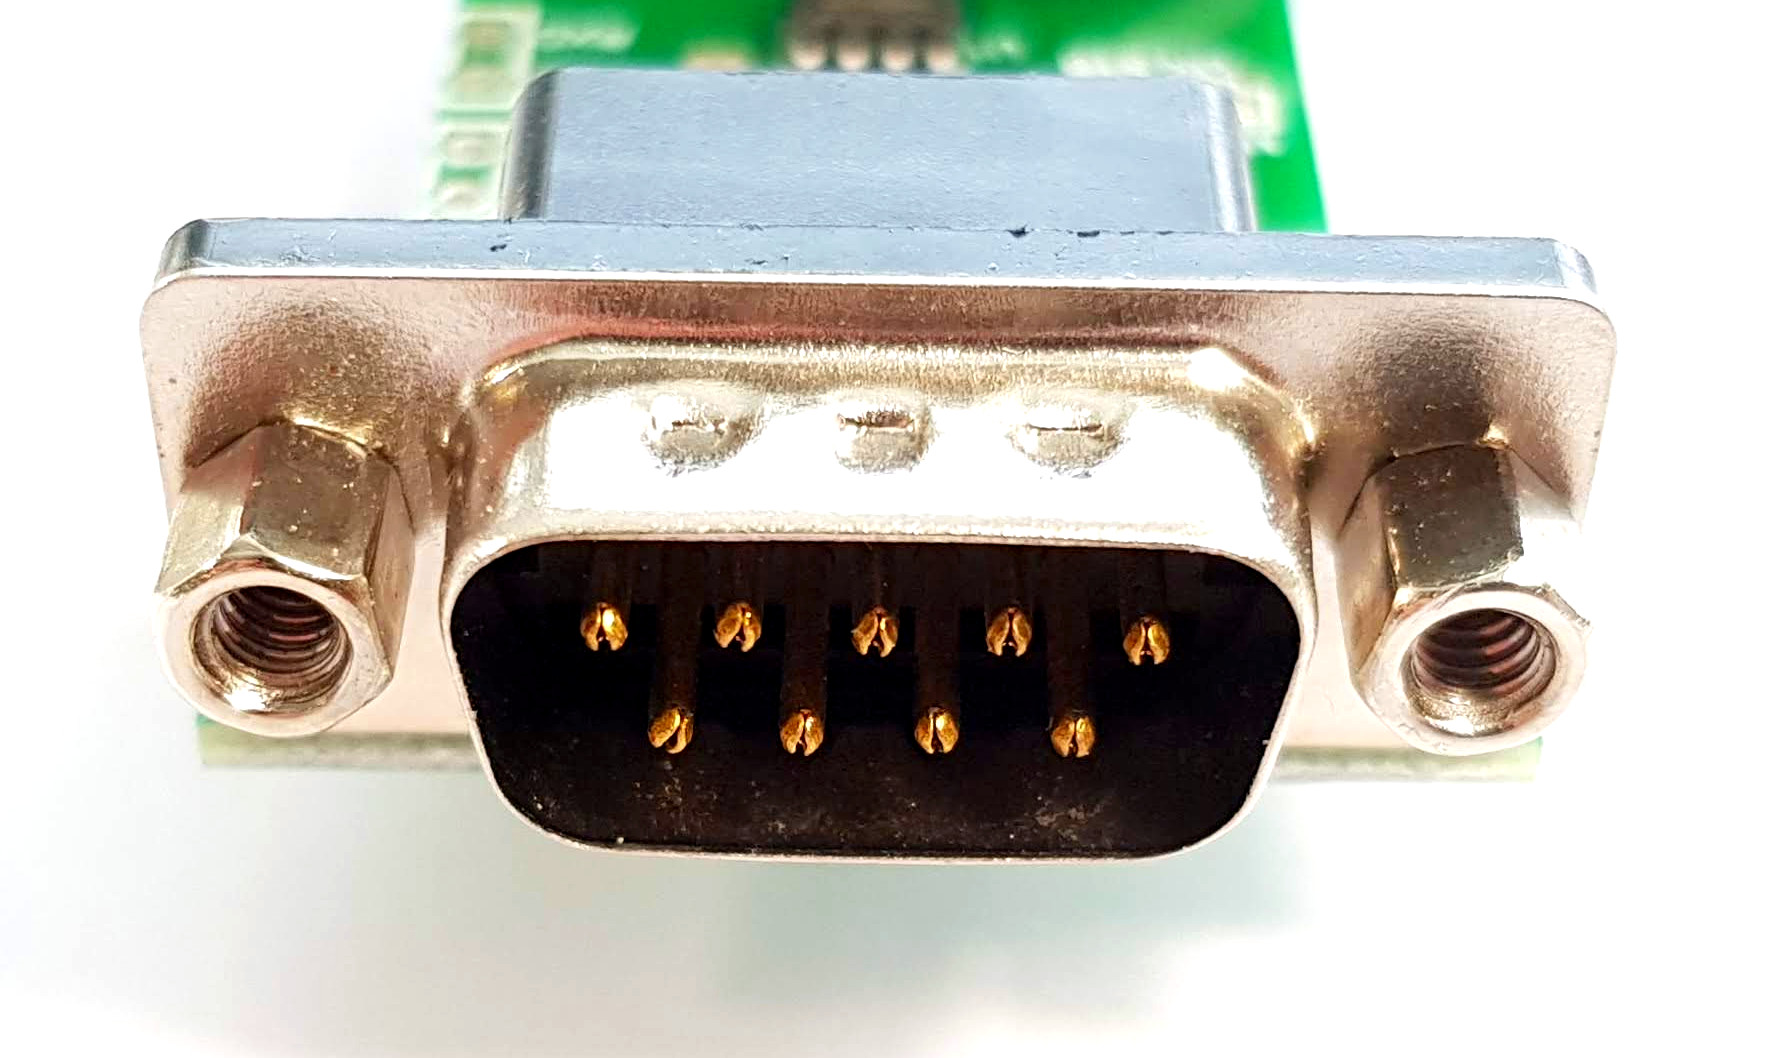
\includegraphics[width=0.35\textwidth]{de-9_connector_male_plug}
    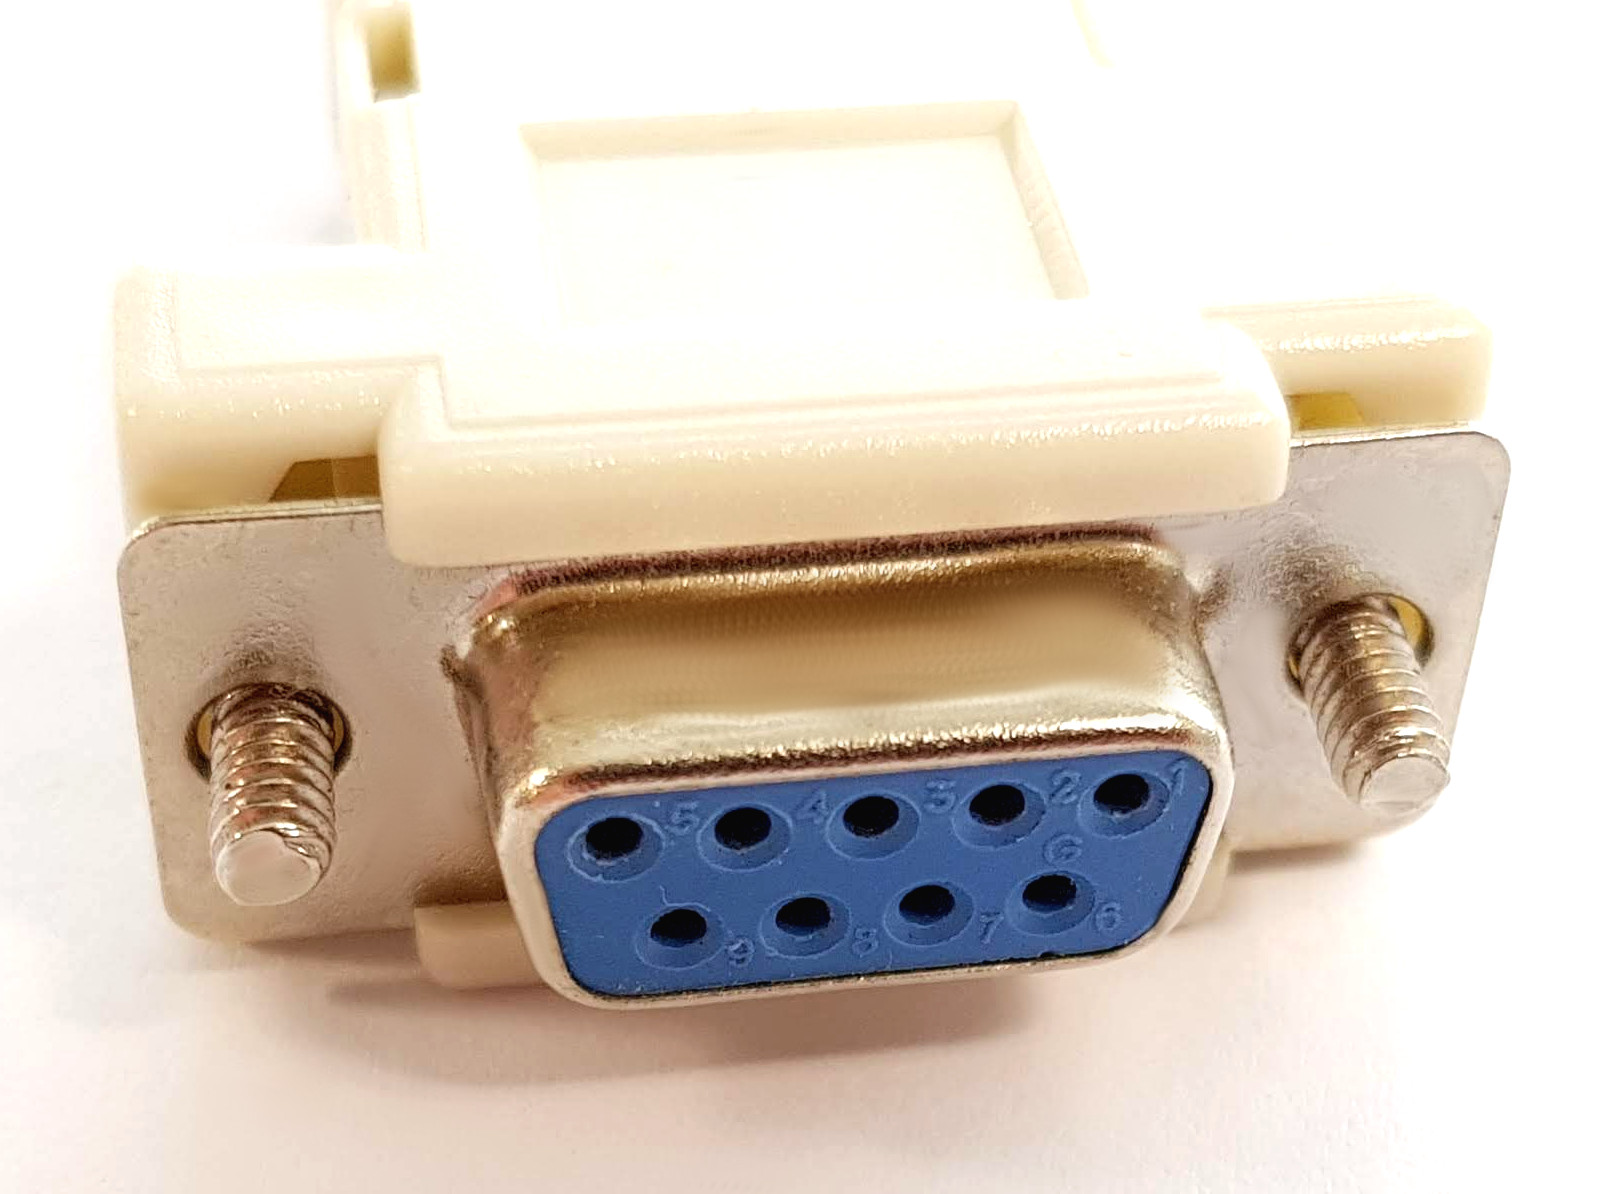
\includegraphics[width=0.35\textwidth]{de-9_cable_female_socket}\\
    Device (left) and cable (right) connectors.
    \caption{UCANPHY D-Sub connectors\label{fig:connector_d_sub}}
\end{figure}

\clearpage  % Enforce \clearpage because the text here is very graphics-heavy and may be hard to read otherwise
\section{UCANPHY M8}

The UCANPHY M8 connector type is based on the generic circular M8 connector type.
This is a popular industry-standard connector; there are multiple vendors that manufacture compatible components:
connectors, cables, termination plugs, T-connectors, and so on.
The pinning, physical layer, and supply voltages used in this connector type are compatible with CiA 103 (CANopen)
and some other CAN bus standards.

{
\NoLeftSkip
\begin{UAVCANCompactTable}{|X[3] X[2]|}
    Advantages & Disadvantages \\
    \begin{itemize}
        \item Compatibility with existing COTS hardware.
        Connectors, cables, termination plugs, and other components can be purchased from many different vendors.
        \item High-reliability options suitable for safety-critical systems are available from multiple vendors.
        \item Low-cost options are available from multiple vendors.
        \item Reasonably compact. M8 connectors are much smaller than D-Sub.
        \item PCB-mounted and panel-mounted types are available.
    \end{itemize}
    &
    \begin{itemize}
        \item M8 connectors may be a poor fit for applications that have severe weight and space constraints.
        \item The level of adoption in the industry is noticeably lower than that of the D-Sub connector type.
    \end{itemize}
\end{UAVCANCompactTable}
}

The UCANPHY M8 connector is based on the \textbf{circular M8 B-coded 5-circuit} connector type\footnote{%
    Do not confuse A-coded and B-coded M8 connectors -- they are not mutually compatible.
}.
Devices are equipped with the male plug mounted on the panel or on the PCB,
and cables are equipped with the female socket on both ends (figure~\ref{fig:connector_m8}).

The CAN physical layer standard that should be used with this connector type is
ISO 11898-2\footnote{Also known as \emph{high-speed CAN}.}.

Devices that deliver power to the bus are required to provide 23.0--30.0 V on the bus power line, 24 V nominal.
Devices that are powered from the bus should expect 18.0--30.0 V on the bus power line.
The current shall not exceed 3 A per connector.

Table~\ref{table:connector_m8_pinout} documents the pinout specification for the UCANPHY M8 connector type.
Wires ``CAN high'' and ``CAN low'' should be a twisted pair.

\begin{UAVCANSimpleTable}{UCANPHY M8 connector pinout}{|l l X|}\label{table:connector_m8_pinout}
    \# & Function           & Note \\
    1  & Bus power supply   & 24 V nominal. See the power supply requirements. \\
    2  & CAN shield         & Optional. \\
    3  & CAN high           & Twisted with ``CAN low'' (pin 4). \\
    4  & CAN low            & Twisted with ``CAN high'' (pin 3). \\
    5  & Ground             & \\
\end{UAVCANSimpleTable}

\begin{figure}[hbt]
    \centering
    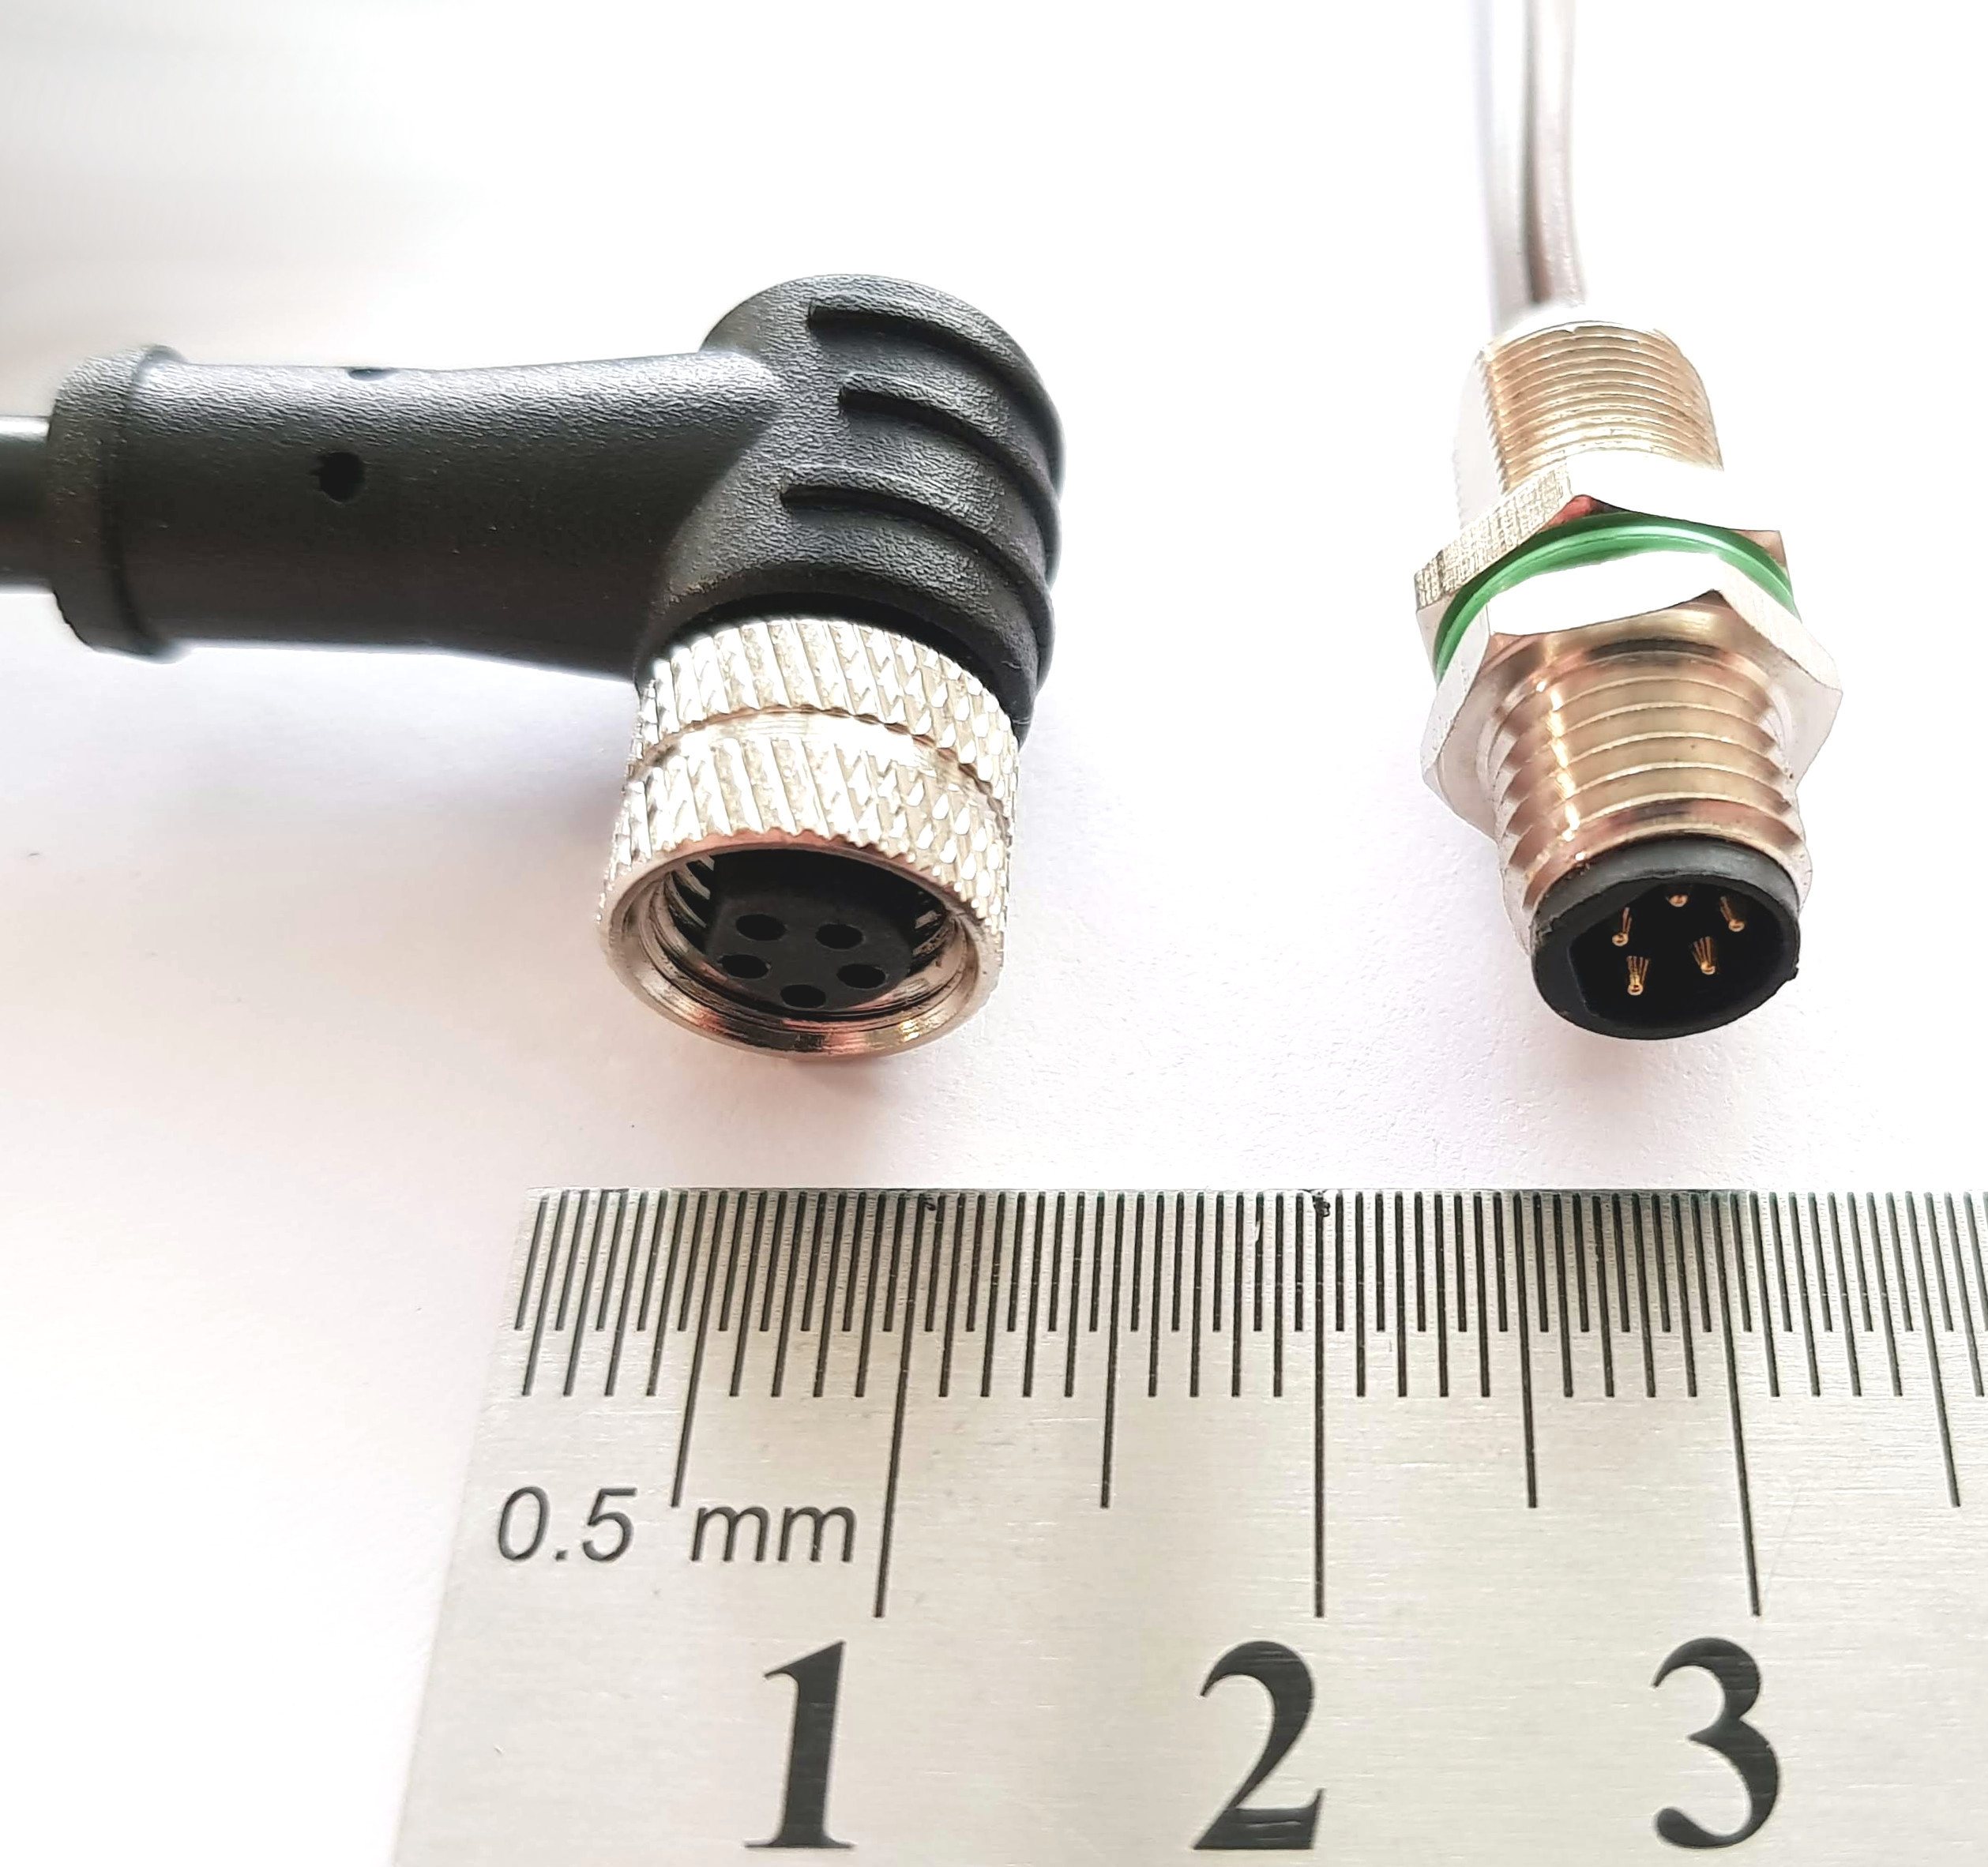
\includegraphics[width=0.35\textwidth]{m8_connector_pair_female_socket_male_plug}
    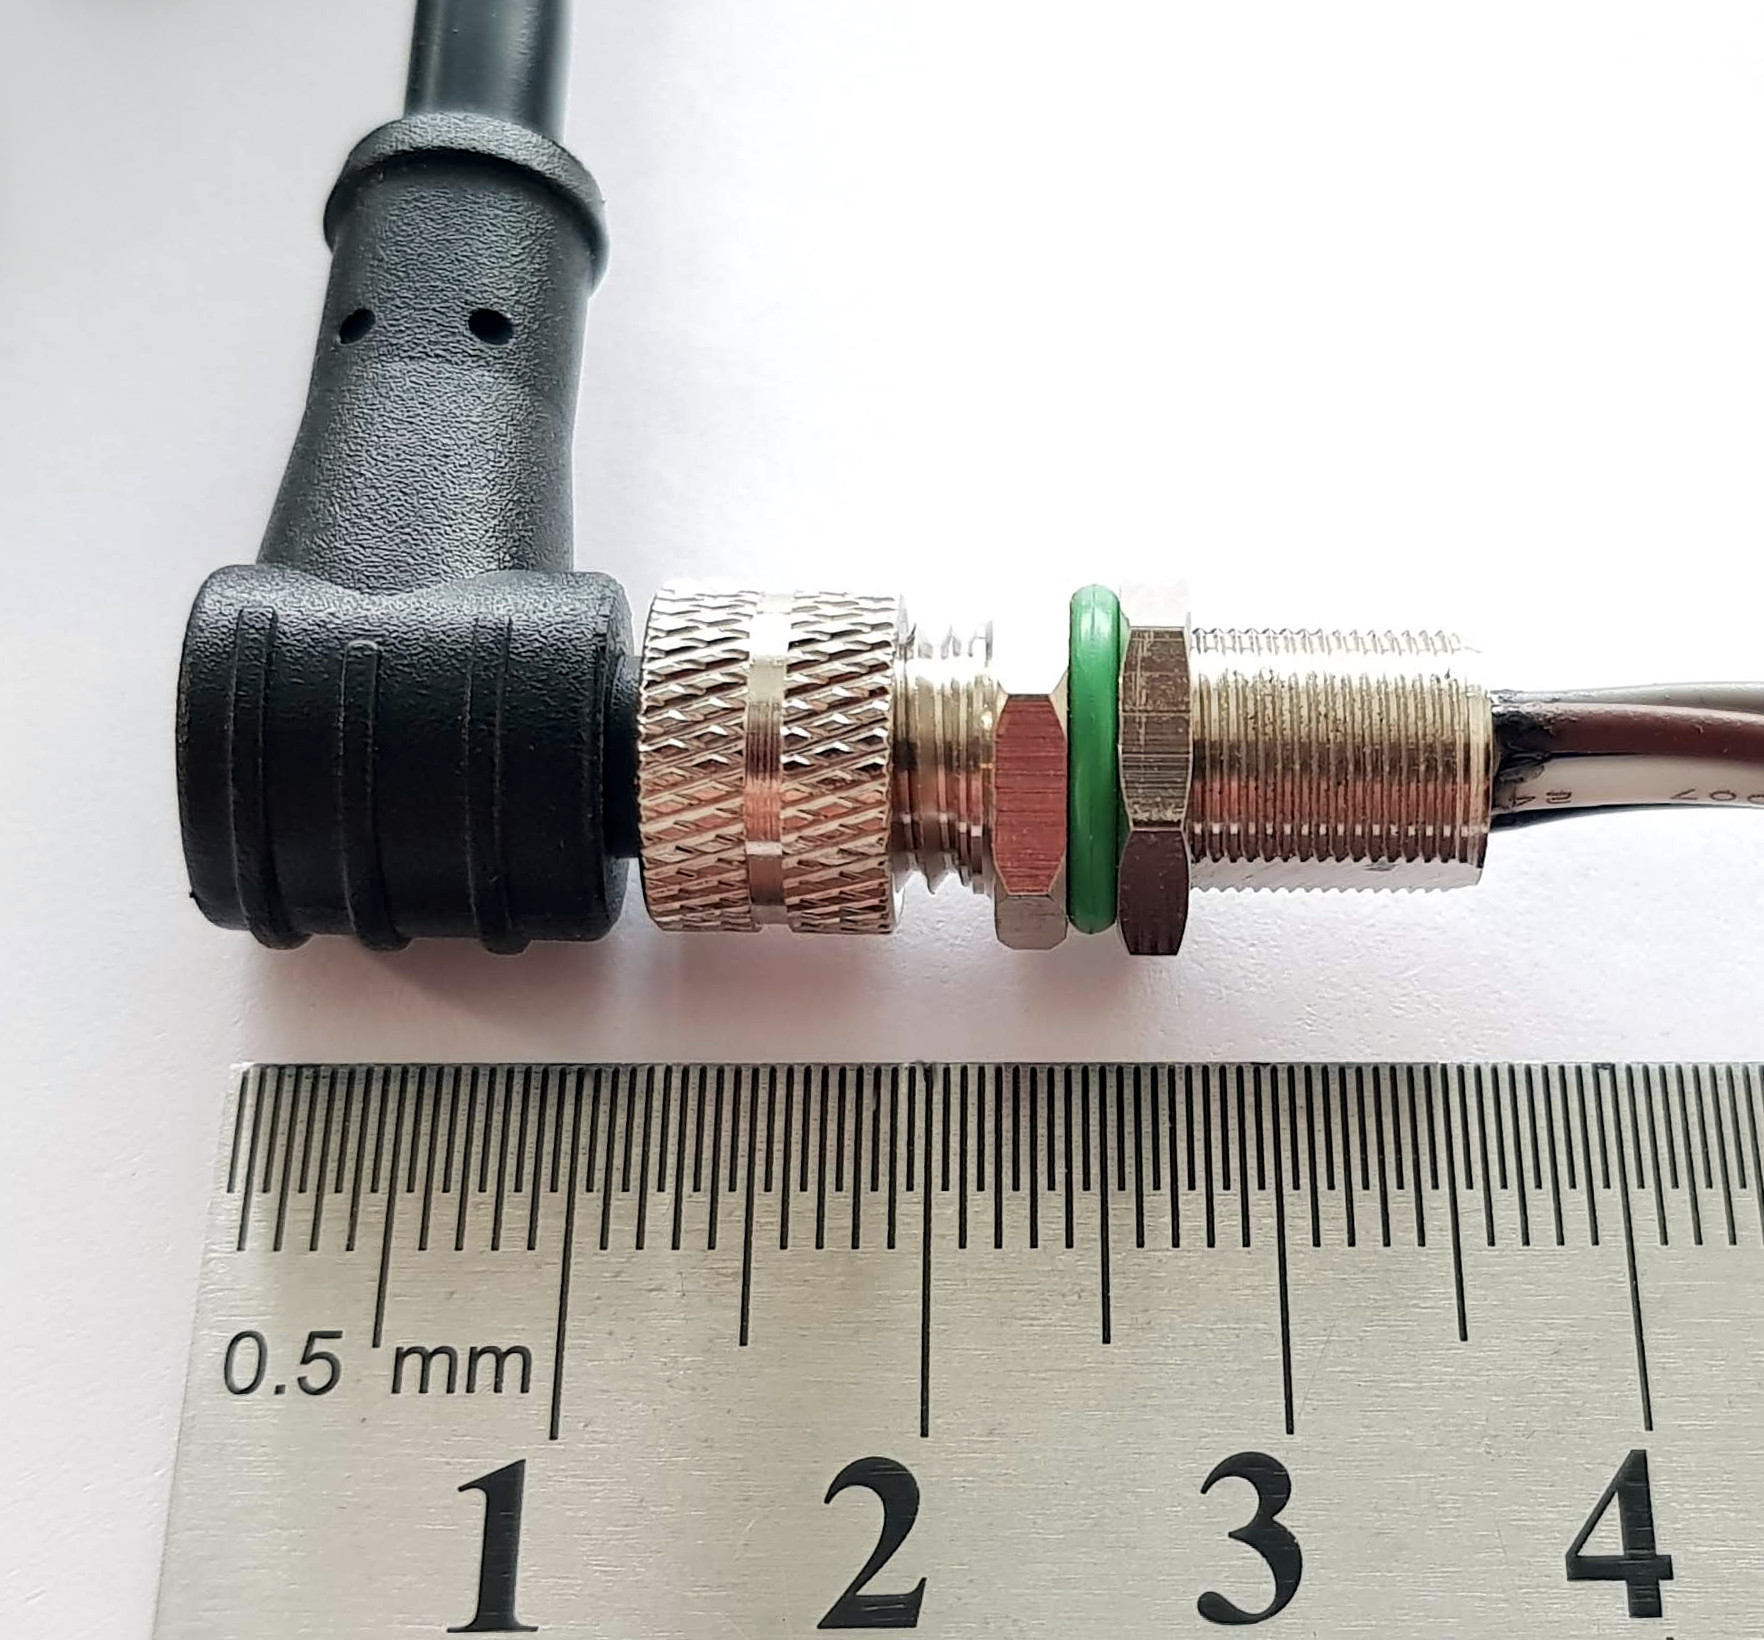
\includegraphics[width=0.35\textwidth]{m8_connector_pair_assembled}\\
    Female socket cable connector, male plug device connector, and the assembled pair.
    \caption{UCANPHY M8 connectors\label{fig:connector_m8}}
\end{figure}

\clearpage  % Enforce \clearpage because the text here is very graphics-heavy and may be hard to read otherwise
\section{UCANPHY Micro}

The UCANPHY Micro connector is intended for weight- and space-sensitive applications.
It is a board-level connector, meaning that it is installed on the PCB rather than on the panel.

The Micro connector is compatible with the Dronecode Autopilot Connector Standard.
This connector type is recommended for small UAV and nanosatellites.
It is also the recommended connector for attaching external panel-mounted connectors
(such as the M8 or D-Sub types) to the PCB inside the enclosure.

{
\NoLeftSkip
\begin{UAVCANCompactTable}{|X X|}
    Advantages & Disadvantages \\
    \begin{itemize}
        \item Extremely compact, low-profile. The PCB footprint is under 9$\times$5 millimeters.
        \item Secure positive lock ensures that the connection will not self-disconnect when exposed to vibrations.
        \item Low cost.
    \end{itemize}
    &
    \begin{itemize}
        \item Board-level connections only. No panel-mounted options available.
        \item No shielding available.
        \item Not suitable for safety-critical hardware.
    \end{itemize}
\end{UAVCANCompactTable}
}

The UCANPHY Micro connector is based on the proprietary \textbf{JST GH 4-circuit} connector type\footnote{%
    The top-entry type is not PCB-footprint-compatible with the side-entry type -- its pin ordering is reversed.
    The wire-side pinout, however, is compatible, so both types can be used interchangeably as long
    as their PCB footprints are correct.
}.

The CAN physical layer standard that can be used with this connector type is ISO 11898-2.

Devices that deliver power to the bus are required to provide 4.9--5.5 V on the bus power line, 5.0 V nominal.
Devices that are powered from the bus should expect 4.0--5.5 V on the bus power line.
The current shall not exceed 1 A per connector.

Table~\ref{table:connector_micro_pinout} documents the pinout specification for the
UCANPHY Micro connector type.
The suitable wire type is \#30 to \#26 AWG, outer insulation diameter 0.8--1.0 mm, multi-strand.
Wires ``CAN high'' and ``CAN low'' shall form a twisted pair.

\begin{UAVCANSimpleTable}{UCANPHY Micro connector pinout}{|l l X|}\label{table:connector_micro_pinout}
    \# & Function           & Note \\
    1  & Bus power supply   & 5 V nominal. See the power supply requirements. \\
    2  & CAN high           & Twisted with ``CAN low'' (pin 3). \\
    3  & CAN low            & Twisted with ``CAN high'' (pin 2). \\
    4  & Ground             & \\
\end{UAVCANSimpleTable}

\begin{figure}[hbt]
    \centering
    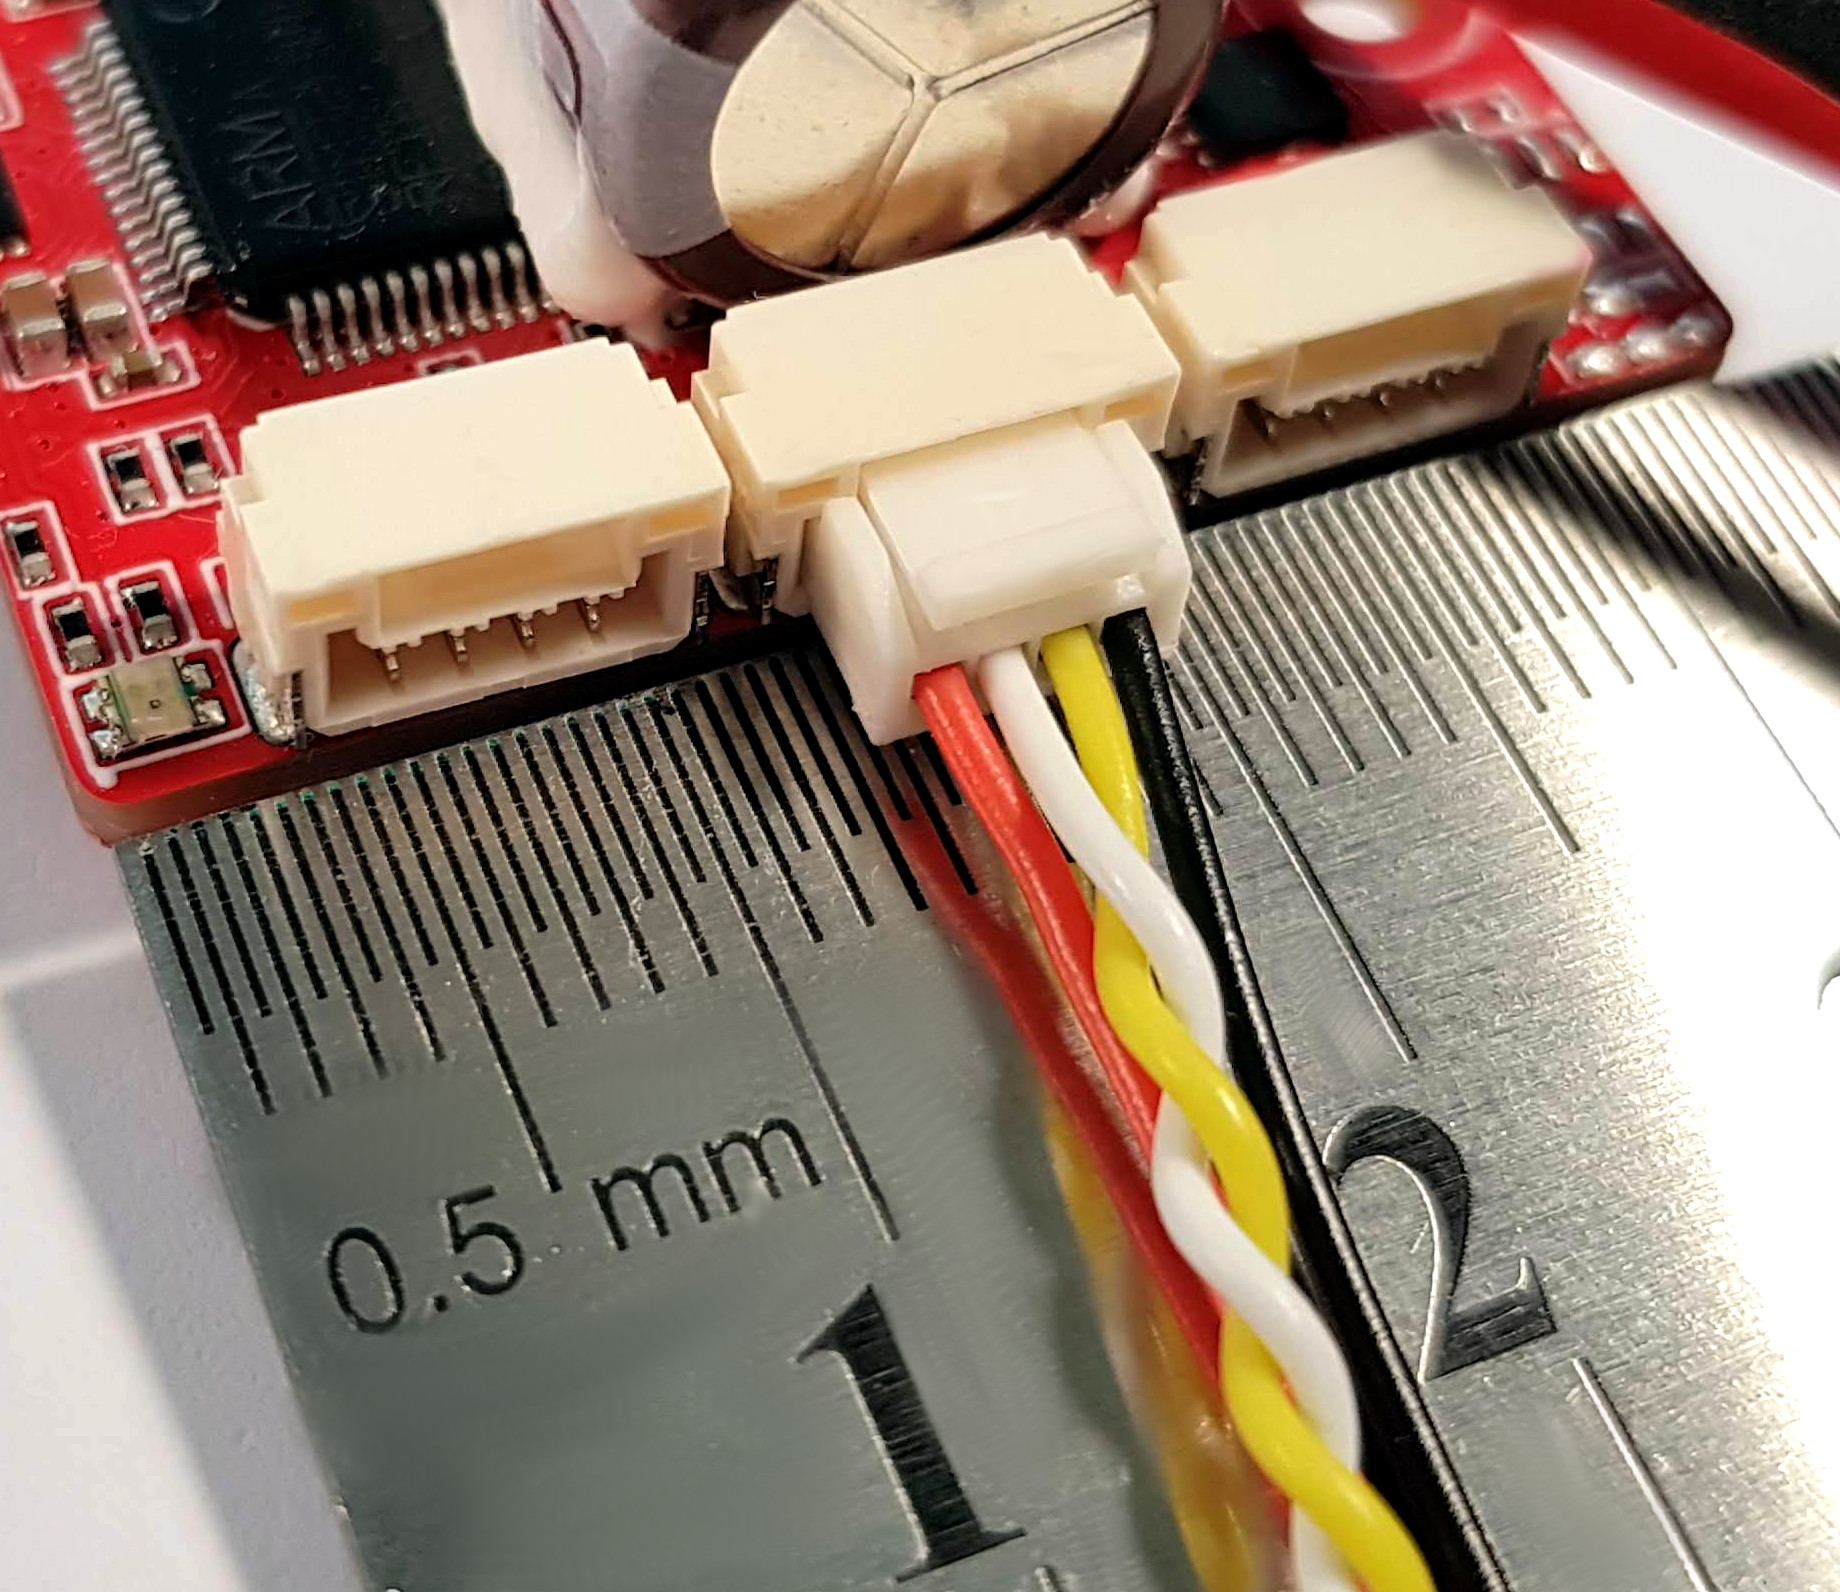
\includegraphics[width=0.35\textwidth]{jst_gh_connectors}
    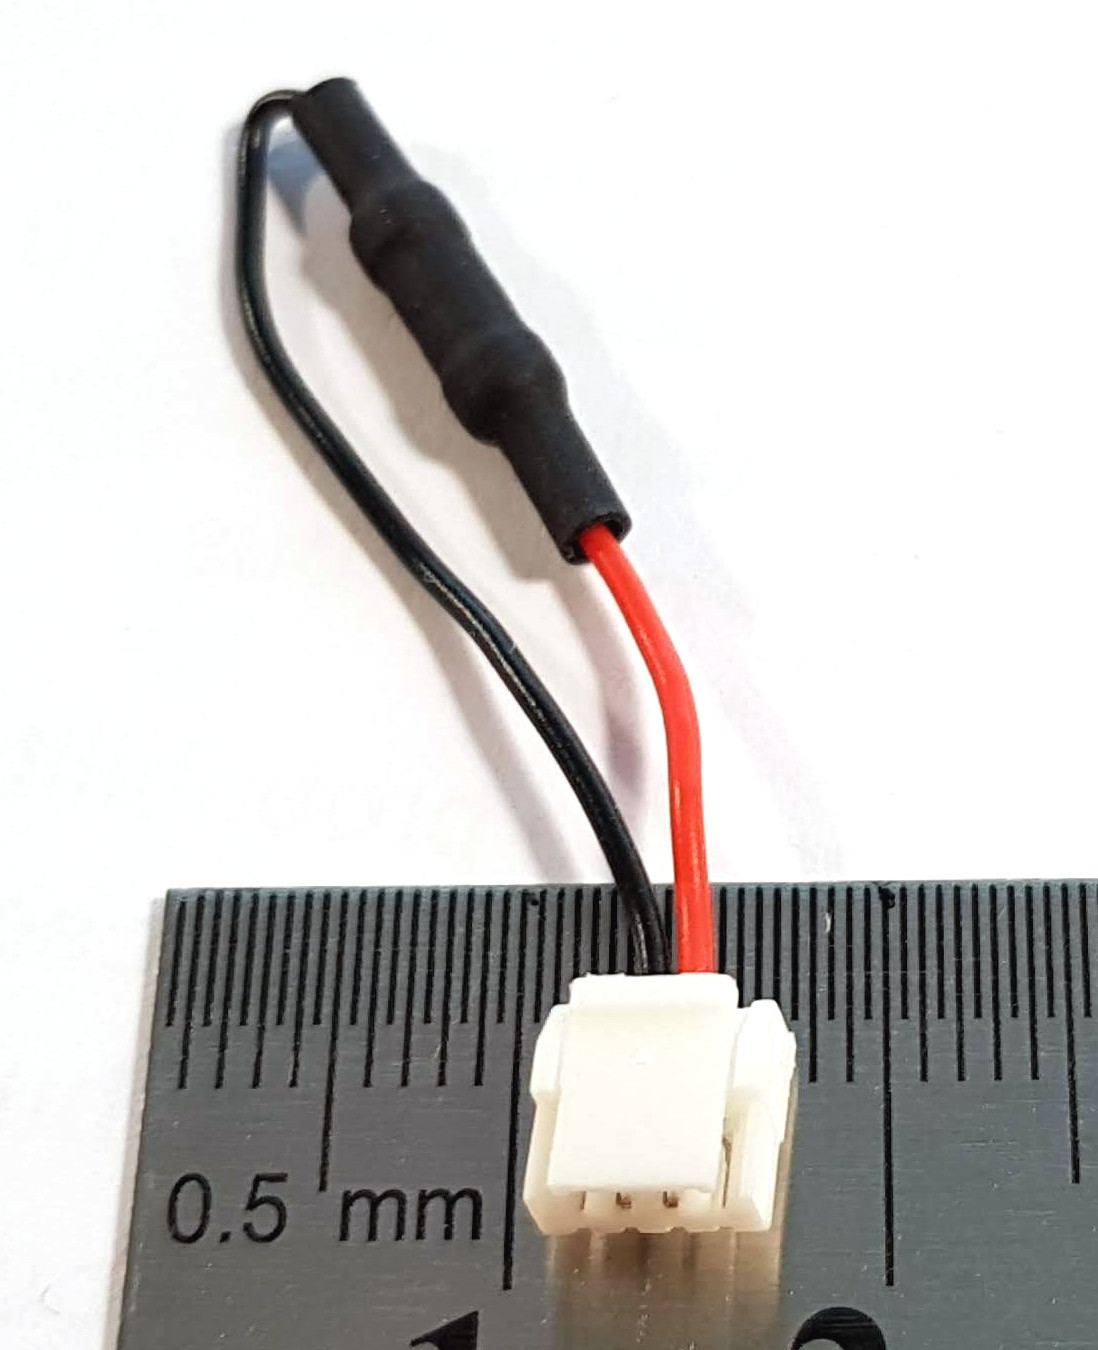
\includegraphics[width=0.30\textwidth]{jst_gh_termination_plug}\\
    Right-angle connector with a twisted pair cable connected; a $120\Omega{}$ termination plug.
    \caption{UCANPHY Micro connectors \label{fig:connector_micro}}
\end{figure}
